
\chapter{Resultados\label{chap:Resultados}}

% Resumo opcional. Comentar se não usar.
%\resumodocapitulo{resumo opcional}

%\section{Resultados}

\section{Teste preliminar} \label{sect:testepreliminar}

Durante testes preliminares, analisou-se a variação dos valores de RSSI e frequência Doppler com uma única TAG e uma única antena. A princípio as leituras pareciam muito sujeitas a ruído e pequenas alterações, então foram aplicados dois filtros: um filtro passa altas com corte em -60dB para o sinal de RSSI e um filtro rejeita banda para frequência Doppler para ignorar leituras menores que -1,50Hz e maiores que 1,50Hz. O teste preliminar resultou na figura \ref{fig:teste_preliminar}.
 
 \begin{figure}[ht]
    \centering
    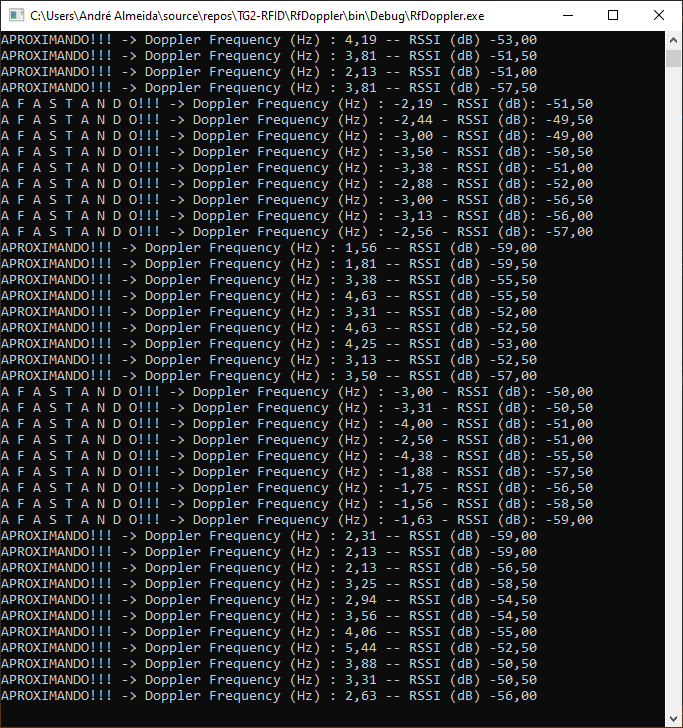
\includegraphics[width=0.7\linewidth]{figs/Metodologia/teste_doppler+RSSI_corte_60db.PNG}
    \caption{Captura de tela mostrando os dados de frequência Doppler e potência RSSI capturados no teste preliminar}
    \label{fig:teste_preliminar}
\end{figure}
 
 O teste se mostrou bastante promissor, pois é possível observar na figura \ref{fig:teste_preliminar} que realizando as configurações corretas e aplicando filtros para rejeitar \textit{outliers} de leitura é possível extrair informações úteis das leituras. Neste teste o valor da frequência Doppler foi observado para definir se a TAG se aproxima ou se afasta da antena.
 
 Ainda é possível perceber que as leituras de frequência Doppler e RSSI, seguem tendências bem definidas. As leituras de frequência Doppler são positivas ao aproximar a TAG da antena, e negativas ao afastar a TAG da antena. A transição entre leituras positivas e negativas ocorre no exato momento de passagem na frente da leitora. As leituras de potência RSSI tentem a ser maiores no momento em que a pessoa está mais próxima da antena, e menores a medida em que se afasta da antena.
 
 Apesar de seguirem uma tendência bem definida, possuem variações abruptas, algumas vezes no sentido oposto ao esperado. Por exemplo, observa-se uma queda abrupta de -51,00 dB e -52,50 dB para -57,00 dB nas duas transições entre o momento em que a pessoa se aproxima e o momento em que a pessoa se afasta da antena. Quanto ao efeito Doppler, este é proporcional à velocidade da pessoa, entretanto, o caminhar de uma pessoa não segue uma velocidade constante a todo momento, e portanto nota-se uma flutuação constante no valor lido.

\section{Teste do programa implementado}

O \textit{software} criado para este trabalho segue a metodologia e as estratégias mencionadas na seção \ref{section:estrategias}. O programa foi desenvolvido de tal forma que, ao mesmo tempo, é possível realizar todos os seis casos de teste. Para isso, a classe \textit{cardholder} possui sete variáveis para armazenar ambientes: uma para o ambiente real - indicado manualmente no terminal do programa quando executado em modo \textit{debug}, para uma pessoa específica apenas - e seis para as suposições de ambiente atual de cada caso de teste.

Um teste foi executado e, durante a execução, o programa armazenou, em tempo real, os dados relevantes de cada leitura de TAG (nome do portador da TAG, número EPC, nome da leitora, número da antena que capturou a leitura, data, horário da captura das informações, ambiente atual, curva de valores de potência RSSI, curva de frequência Doppler e as seis hipóteses de ambiente atual geradas pelos casos de teste). Estes dados podem ser vistos no anexo \ref{anex:testlog}.

Durante a execução do teste, uma pessoa transitou pelo ambiente do LARA, enquanto outra registrava manualmente os valores de ambiente real (anexo \ref{anex:testlog}).

As figuras \ref{fig:cruzamento01}, \ref{fig:cruzamento10}, \ref{fig:cruzamento12}, \ref{fig:cruzamento21}, \ref{fig:cruzamento13} e \ref{fig:cruzamento31} mostram imagens dos vídeos gravados, durante os cruzamentos de fronteira entre ambientes, em frente às leitoras e às antenas.


\begin{figure}[H]
    \centering
    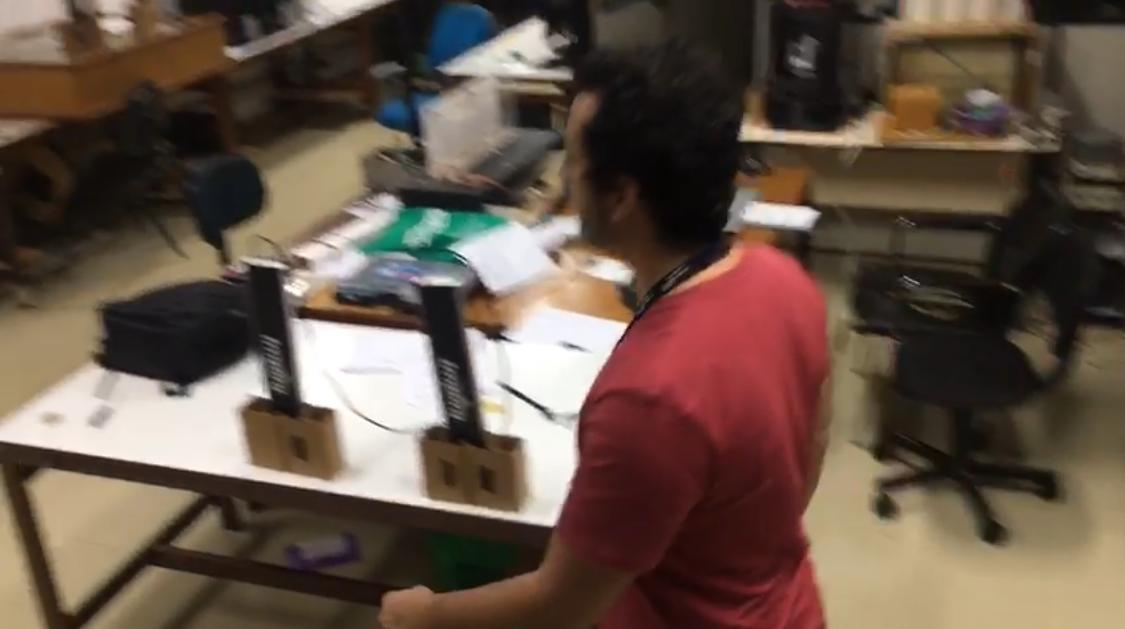
\includegraphics[width=0.5\linewidth]{figs/Resultados/cruzamento01.jpeg}
    \caption{Teste do programa - Leitura do cruzamento da fronteira de Área Externa (0) para Sala Principal (1)}
    \label{fig:cruzamento01}
\end{figure}

\begin{figure}[H]
    \centering
    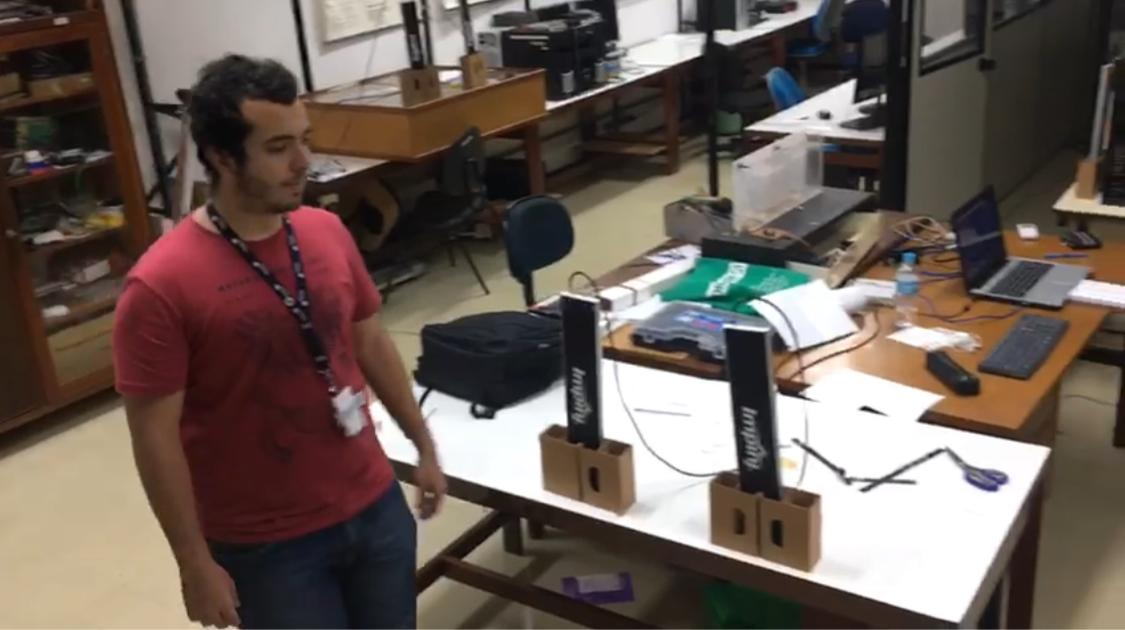
\includegraphics[width=0.5\linewidth]{figs/Resultados/cruzamento10.jpeg}
    \caption{Teste do programa - Leitura do cruzamento da fronteira de Sala Principal (1) para Área Externa (0)}
    \label{fig:cruzamento10}
\end{figure}

\begin{figure}[H]
    \centering
    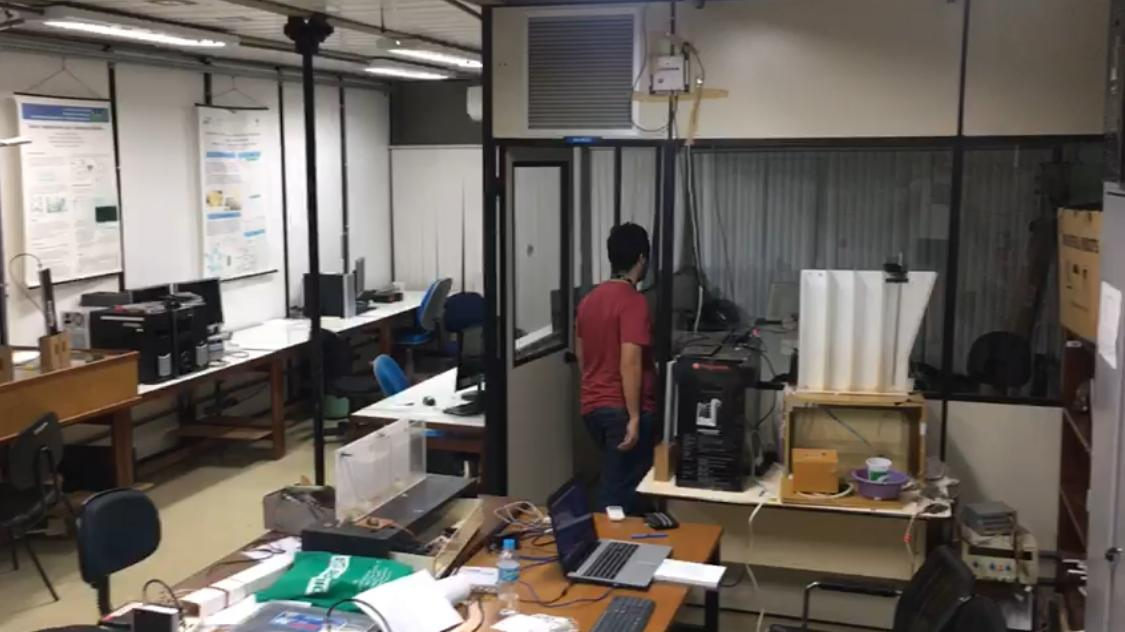
\includegraphics[width=0.5\linewidth]{figs/Resultados/cruzamento12.jpeg}
    \caption{Teste do programa - Leitura do cruzamento da fronteira de Sala Principal (1) para Sala de Reuniões (2)}
    \label{fig:cruzamento12}
\end{figure}

\begin{figure}[H]
    \centering
    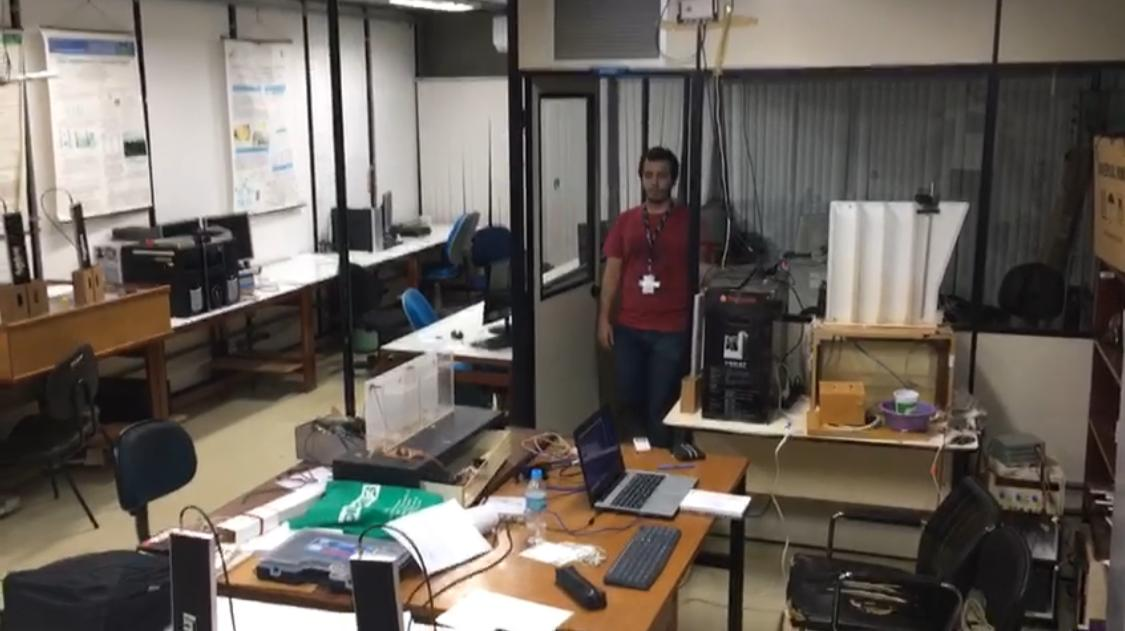
\includegraphics[width=0.5\linewidth]{figs/Resultados/cruzamento21.jpeg}
    \caption{Teste do programa - Leitura do cruzamento da fronteira de Sala de Reuniões (2) para Sala Principal (1)}
    \label{fig:cruzamento21}
\end{figure}

\begin{figure}[H]
    \centering
    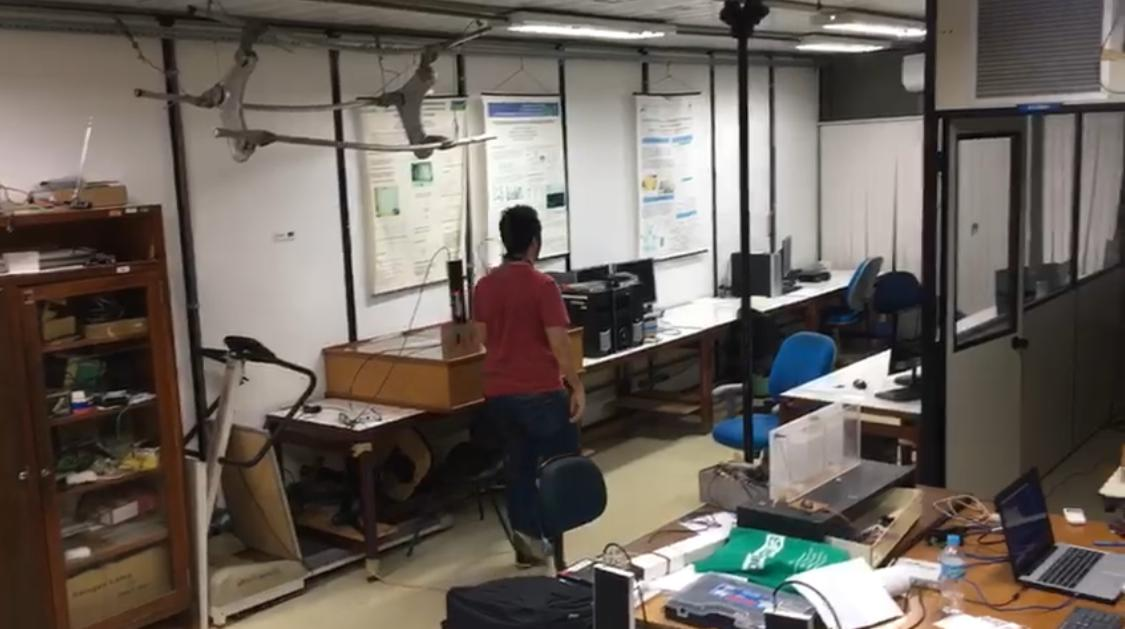
\includegraphics[width=0.5\linewidth]{figs/Resultados/cruzamento13.jpeg}
    \caption{Teste do programa - Leitura do cruzamento da fronteira de Sala Principal (1) para Corredor Baias(3)}
    \label{fig:cruzamento13}
\end{figure}

\begin{figure}[H]
    \centering
    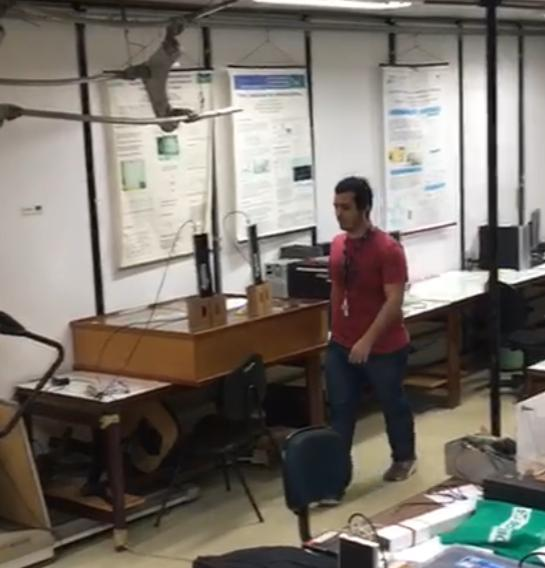
\includegraphics[width=0.5\linewidth]{figs/Resultados/cruzamento31.jpeg}
    \caption{Teste do programa - Leitura do cruzamento da fronteira de Corredor Baias(3) para Sala Principal (1)}
    \label{fig:cruzamento31}
\end{figure}

\section{Eficiência dos métodos}

Cada método de decisão de localização a seguir foi analisado manualmente de acordo com os dados gerados no anexo \ref{anex:testlog}. O critério para contabilizar um erro foi um método apresentar a sala incorreta mais de um minuto após a transição de ambientes ser contabilizada, ou até a próxima mudança de ambientes, o que ocorresse primeiro.

\subsection{Comparação do último valor de RSSI} \label{section:ultimovalorRES}

A eficiência do critério de último valor de RSSI baseada no caso de teste do anexo \ref{anex:testlog} pode ser vista na tabela \ref{tab:resultados1}

\begin{table}[H]
\centering
\caption{Eficiência do critério do último valor com base no teste do anexo \ref{anex:testlog} }
\label{tab:resultados1}
\begin{tabular}{p{5cm} p{5cm}}
\hline
\multicolumn{2}{c}{\cellcolor{lightgray}{Eficiência do critério: Último valor de RSSI}} \\ \hline
Erros confirmados          &  $0 /10$        \\
Confiabilidade & $100\%$ \\ \hline
\end{tabular}
\end{table}

Foram contabilizadas 10 transições e em todas elas, após no máximo quatro leituras, o presente método acertou o ambiente em que a pessoa se encontrava. O programa utiliza a localização de cada \textit{cardholder} para contabilizar todas as pessoas em cada ambiente.


\subsection{Comparação dos tempos dos últimos picos de RSSI} \label{setion:resultRSSIpeak}

A eficiência do critério dos tempos de pico de RSSI baseada no caso de teste do anexo \ref{anex:testlog} pode ser vista na tabela \ref{tab:resultados2}

\begin{table}[H]
\centering
\caption{Eficiência do critério dos tempos de picos de RSSI com base no teste do anexo \ref{anex:testlog} }
\label{tab:resultados2}
\begin{tabular}{p{5cm} p{5cm}}
\hline
\multicolumn{2}{c}{\cellcolor{lightgray}{Eficiência do critério: Tempos de pico de RSSI}} \\ \hline
Erros confirmados          &  $0 / 10$        \\
Confiabilidade & $100\%$ \\ \hline
\end{tabular}
\end{table}

Os itens de erro e confiabilidade desta tabela são os mesmos do caso de teste de último valor, seção \ref{section:ultimovalorRES}, já que foram executados no mesmo teste. Foram 10 transições de ambiente e nenhuma se encontrou equivocada após quatro leituras.

\begin{figure}[H]
    \centering
    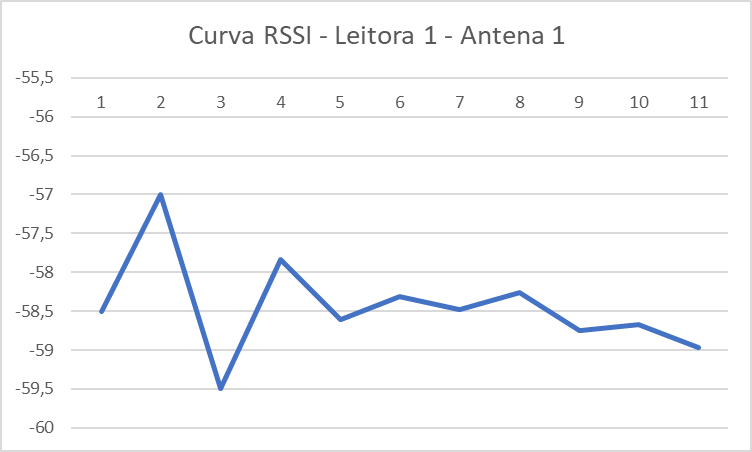
\includegraphics[width=0.8\linewidth]{figs/Resultados/image001.png}
    \caption{\textit{Snapshot} de uma curva de valores RSSI no momento de uma transição - Curva da Leitora 1, Antena 1}
    \label{fig:tranRSSI11}
\end{figure}

\begin{figure}[H]
    \centering
    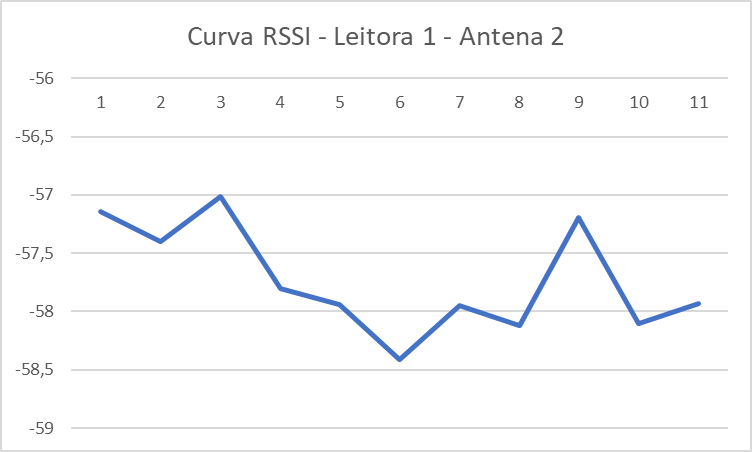
\includegraphics[width=0.8\linewidth]{figs/Resultados/image002.png}
    \caption{\textit{Snapshot} de uma curva de valores RSSI no momento de uma transição - Curva da Leitora 1, Antena 2}
    \label{fig:tranRSSI12}
\end{figure}

As figuras \ref{fig:tranRSSI11} e \ref{fig:tranRSSI12} apresentam os gráficos de uma transição pelo critério dos picos RSSI. É possível observar o pico na curva da antena 2 (figura \ref{fig:tranRSSI12}) no tempo 9 mais recente do que o último pico da antena 1 (figura \ref{fig:tranRSSI11}), caracterizando uma passagem do lado da antena 2. Neste caso específico, realiza-se uma transição do Ambiente Externo (0) para a Sala Principal (1).



\subsection{Comparação da média dos valores de RSSI}

A eficiência do critério média dos valores de RSSI baseada no caso de teste do anexo \ref{anex:testlog} pode ser vista na tabela \ref{tab:resultados3}

\begin{table}[H]
\centering
\caption{Eficiência do critério da média dos valores de RSSI com base no teste do anexo \ref{anex:testlog} }
\label{tab:resultados3}
\begin{tabular}{p{5cm} p{5cm}}
\hline
\multicolumn{2}{c}{\cellcolor{lightgray}{Eficiência do critério: Média dos valores de RSSI}} \\ \hline
Erros confirmados          &  $6 / 10$        \\
Confiabilidade & $40\%$ \\ \hline
\end{tabular}
\end{table}

O comparador de médias acertou 4 transições, entretanto, na maioria das transições, apresentou o valor errado. Analisando os dados gerados, acredita-se que o modo de funcionamento do programa, que mantém as curvas salvas indefinidamente, são facilmente enganadoras para este método. Ao passar por uma transição e, em um segundo momento, retornar, enquanto não houverem leituras suficientes para sobrescrever os dados das curvas, a média dos dados será muito próxima à ultima passagem. É necessário permanecer imóvel em frente a um par de antenas, obtendo leituras em ambas, para que a curva seja sobrescrita, e o método registre a transição.

\subsection{Comparação da mediana dos sinais RSSI}

A eficiência do critério mediana dos valores de RSSI baseada no caso de teste do anexo \ref{anex:testlog} pode ser vista na tabela \ref{tab:resultados4}

\begin{table}[H]
\centering
\caption{Eficiência do critério da mediana dos valores de RSSI com base no teste do anexo \ref{anex:testlog} }
\label{tab:resultados4}
\begin{tabular}{p{5cm} p{5cm}}
\hline
\multicolumn{2}{c}{\cellcolor{lightgray}{Eficiência do critério: Mediana dos valores de RSSI}} \\ \hline
Erros confirmados          &  $7 / 10$        \\
Confiabilidade & $30\%$ \\ \hline
\end{tabular}
\end{table}

Os itens de erro e confiabilidade desta tabela são os similares aos resultados do caso de testes de média. Nenhum dos dois métodos foi considerado um método confiável ou aplicável.

\subsection{Comparação da travessia por Efeito Doppler}


A eficiência do critério de travessia por Efeito Doppler baseada no caso de teste do anexo \ref{anex:testlog} pode ser vista na tabela \ref{tab:resultados5}

\begin{table}[H]
\centering
\caption{Eficiência do critério de travessia por Efeito Doppler com base no teste do anexo \ref{anex:testlog} }
\label{tab:resultados5}
\begin{tabular}{p{5cm} p{5cm}}
\hline
\multicolumn{2}{c}{\cellcolor{lightgray}{Eficiência do critério: Travessia por efeito Doppler}} \\ \hline
Erros confirmados          &  $3 / 10$        \\
Confiabilidade & $70\%$ \\ \hline
\end{tabular}
\end{table}

O caso de testes de contabilização de transição entre ambientes por efeito Doppler possui resultados que o classificam como um estimador fazível, e que se deve levar em consideração. Entretanto, mostrou-se mais suscetível a erros causados por escarces de leituras. É válido um estudo mais aprofundado neste método, em um trabalho futuro, pois é um método promissor.

\begin{figure}[H]
    \centering
    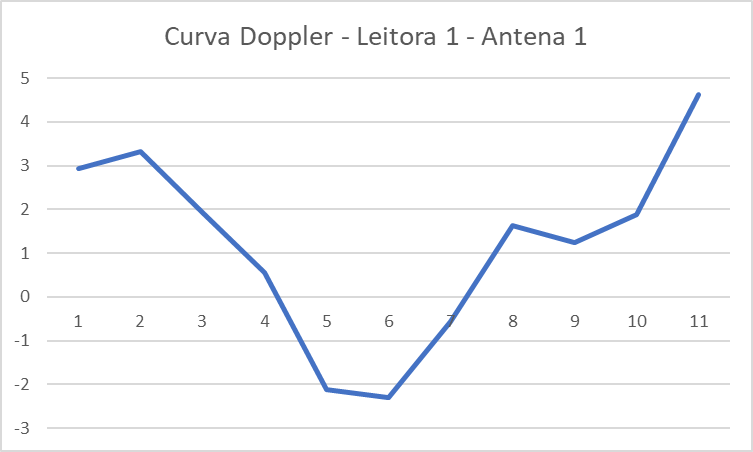
\includegraphics[width=0.8\linewidth]{figs/Resultados/image003.png}
    \caption{\textit{Snapshot} de uma curva de frequências Doppler no momento de uma transição - Curva da Leitora 1, Antena 1}
    \label{fig:tranDoppler11}
\end{figure}

\begin{figure}[H]
    \centering
    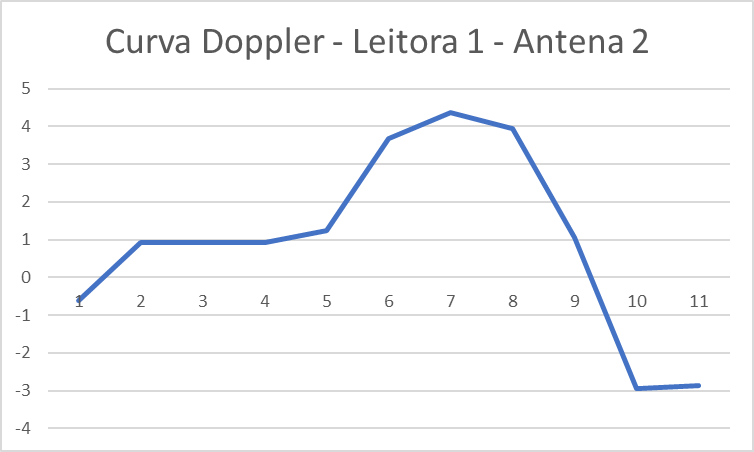
\includegraphics[width=0.8\linewidth]{figs/Resultados/image004.png}
    \caption{\textit{Snapshot} de uma curva de frequências Doppler no momento de uma transição - Curva da Leitora 1, Antena 2}
    \label{fig:tranDoppler12}
\end{figure}

As figuras \ref{fig:tranDoppler11} e \ref{fig:tranDoppler12} apresentam duas curvas de frequências Doppler no momento da mesma transição observada nas figuras \ref{fig:tranRSSI11} e  \ref{fig:tranRSSI12}. É possível observar as transições positivo $\rightarrow$ negativo, no tempo 4 para a antena 1 e no tempo 9 para a antena 2, o que indica uma movimentação do Ambiente Externo (0) para a Sala Principal (1), como no caso da seção \ref{setion:resultRSSIpeak}. É interessante observar que estes são os mesmos tempos onde são observadas as curvas de pico do método que utiliza os valores de RSSI.


\subsection{Combinação da técnica de picos de RSSI com Efeito Doppler}

A eficiência do critério de travessia por tempos de pico RSSI e  Efeito Doppler baseada no caso de teste do anexo \ref{anex:testlog} pode ser vista na tabela \ref{tab:resultados6}

\begin{table}[H]
\centering
\caption{Eficiência do critério de combinação de comparação de picos de valores de RSSI e travessia por Efeito Doppler com base no teste do anexo \ref{anex:testlog} }
\label{tab:resultados6}
\begin{tabular}{p{5cm} p{5cm}}
\hline
\multicolumn{2}{c}{\cellcolor{lightgray}{Eficiência do critério: Travessia por efeito Doppler}} \\ \hline
Erros confirmados          &  $3 / 10$        \\
Confiabilidade & $70\%$ \\ \hline
\end{tabular}
\end{table}

Este método, da maneira como foi implementado, nivela os dois métodos de que é composto pelo pior desempenho. Isso se deve ao modo como foi implementado, aplicando-se a lógica "E" para combinar as sugestões de transição dos dois métodos. O teste com a combinação proporcional dos dois métodos, combinando os pesos para cada critério baseado nas suas respectivas eficiências.